% Supplementary Material for AdaScale (ICASSP 2027 submission)
\documentclass[10pt]{article}
\usepackage[margin=0.9in]{geometry}
\usepackage{amsmath,amssymb,graphicx,booktabs}
\usepackage{algorithm}
\usepackage[noend]{algpseudocode}
\usepackage[font=small]{caption}
\usepackage[hidelinks]{hyperref}

\newcommand{\ourfig}[2]{\begin{figure}[t]\centering
\includegraphics[width=#1\linewidth]{#2}\end{figure}}
\title{Supplementary Material\\ for ``AdaScale: Diagnosing and Adapting Multi-Scale Fusion\\ for Training-Free Zero-Shot Recognition''}
\author{Dongxu Liu$^{1,\ast}$, Keming Fan$^{2}$, Xiang Luo$^{3}$, Chenrui Zhu$^{3}$, Dongyang Liu$^{4}$\\
$^{1}$School of Artificial Intelligence, Jilin University, Changchun, China\\
$^{2}$College of Computer Science and Technology, Jilin University, Changchun, China\\
$^{3}$College of Software, Jilin University, Changchun, China\\
$^{4}$Yingcai Honors College, University of Electronic Science and Technology of China, Chengdu, China\\
$^{\ast}$Corresponding author: liudx9924@mails.jlu.edu.cn}
\date{}

\begin{document}
\maketitle
\vspace{-2em}

\section{Implementation Details}
\label{s:impl}

\paragraph{Multi-scale feature extraction.}
For each dataset we extract 10 per-scale feature sets following the
reference LG-CLIP pipeline~\cite{shi2026lgclip}: each test image is cropped
by \texttt{RandomResizedCrop}$(224, \text{scale}=(s/10, s/10))$ with BICUBIC
interpolation and CLIP normalization, then encoded by the frozen CLIP image
encoder into an L2-normalized feature. Per-scale features are stored as HDF5
files; text prototypes use the template ``A photo of a $\{$class$\}$.''.
Script: \texttt{third\_party/LG-CLIP/vanilla\_clip\_ms.py}; all evaluation is
training-free and gradient-free.

\paragraph{CUB-200-2011.}
Official train/test split (5{,}794 test images, 200 classes); class names
cleaned as in the reference pipeline. Only text prototypes are evaluated on
CUB (synthetic prototypes require offline per-class image generation and are
covered by the other three datasets).

\paragraph{Frozen hyperparameters.}
Early-exit $r{=}4$, $\delta{=}0.65$, $\varepsilon{=}0.01$; selector
$\theta{=}0.01$, $n{=}500$ unlabeled calibration samples drawn from the target test pool (labels never used); soft-fusion
temperature $\tau_s{=}0.02$. \textbf{None of these is tuned on test labels};
configurations were fixed from the calibration-side search reported in
Sec.~\ref{s:select} and Sec.~\ref{s:extra}.

\section{AdaScale Algorithm}
\label{s:algo}

\begin{algorithm}[t]
\caption{AdaScale: hierarchical training-free controller}
\begin{algorithmic}[1]
\Require test image $x$; unlabeled calibration set $\mathcal{U}$ ($n{=}500$);
frozen config $(\theta, r, \delta, \varepsilon, \tau_s)$; prototypes $P$.
\State Compute fused and largest-scale predictions on $\mathcal{U}$;
$\Delta H \gets \frac{1}{n}\sum_i \frac{H(p^{\text{fused}}_i)-H(p^{\text{single}}_i)}{\log C}$
\If{$\Delta H > \theta$} \Comment{Level 1: target-domain fusion diagnosis}
    \State \textbf{return} largest-scale prediction \Comment{\textsc{Single}: 1 forward}
\Else \Comment{\textsc{Fused}: Level 2 loop}
    \State $\mathcal{V} \gets \emptyset$; prefix $\gets 0$
    \For{$t = 1,\dots,10$}
        \State $f_t \gets \mathrm{Encode}(\mathrm{RRC}(x, t/10))$;
        $\mathcal{V} \gets \mathcal{V} \cup \{t\}$
        \State $p^{(t)} \gets \mathrm{softmax}(\mathrm{prefix})$ \Comment{prefix fusion}
        \If{$t \ge r$ \textbf{and} $\arg\max p^{(t-j)}$ equal for $j{=}0..r{-}1$
            \textbf{and} $m_t \ge \delta$ \textbf{and} $D_{\mathrm{JS}}(p^{(t)}\|p^{(t-1)}) \le \varepsilon$}
            \State \textbf{break} \Comment{sample-wise exit}
        \EndIf
    \EndFor
    \State \textbf{return} $\arg\max_c \sum_{s \in \mathcal{V}} s \cdot
    \mathrm{softmax}\!\left(f_s^\top P / \tau_s\right)_c$
    \Comment{probability-level soft fusion}
\EndIf
\end{algorithmic}
\end{algorithm}

\section{Selector Sensitivity Analysis}
\label{s:select}

The Level-1 decision uses a single scalar on unlabeled data. Its
robustness was verified as follows.
\begin{itemize}
\item \textbf{Calibration sub-sampling}: 200 uniform sub-samples of size
$n{=}500$ per setting produced the same \textsc{Single}/\textsc{Fused}
decision as the full set in 98--100\% of runs (100\% at $n{=}1000$).
\item \textbf{Threshold tolerance}: the decision is invariant for
$\theta \in [0.5\%, 2.3\%]$; the observed $\Delta H$ gap between regimes is
$+2.20$pp (minimum \textsc{Single}-side value $+2.66\%$ at EuroSAT/gen,
maximum \textsc{Fused}-side value $+0.46\%$ at Flowers/gen).
\item \textbf{Cross-backbone}: 11/11 correct decisions across CLIP
ViT-B/32 and ViT-B/16 (Table~\ref{tab:b16} and main Table~III).
\item \textbf{Failure mode is safe}: a wrong \textsc{Fused} decision would
forfeit compute savings but keep full-fusion accuracy.
\end{itemize}

\section{Additional Diagnostics}
\label{s:diag}

\paragraph{Prefix dynamics.}
Figure~\ref{fig:traj} shows prefix decision margin and entropy trajectories
grouped by execution outcome on the four FUSED settings (ViT-B/32).
Early-exit samples stabilize fast (margin $\approx 0.9$ after 3--4 scales);
full-run correct samples remain at intermediate margin ($\approx 0.3$);
full-run wrong samples have the lowest margin ($\approx 0.2$) and the
highest entropy throughout --- the stopping rule separates exactly the
regimes it is designed to separate.

\begin{figure}[t]
\centering
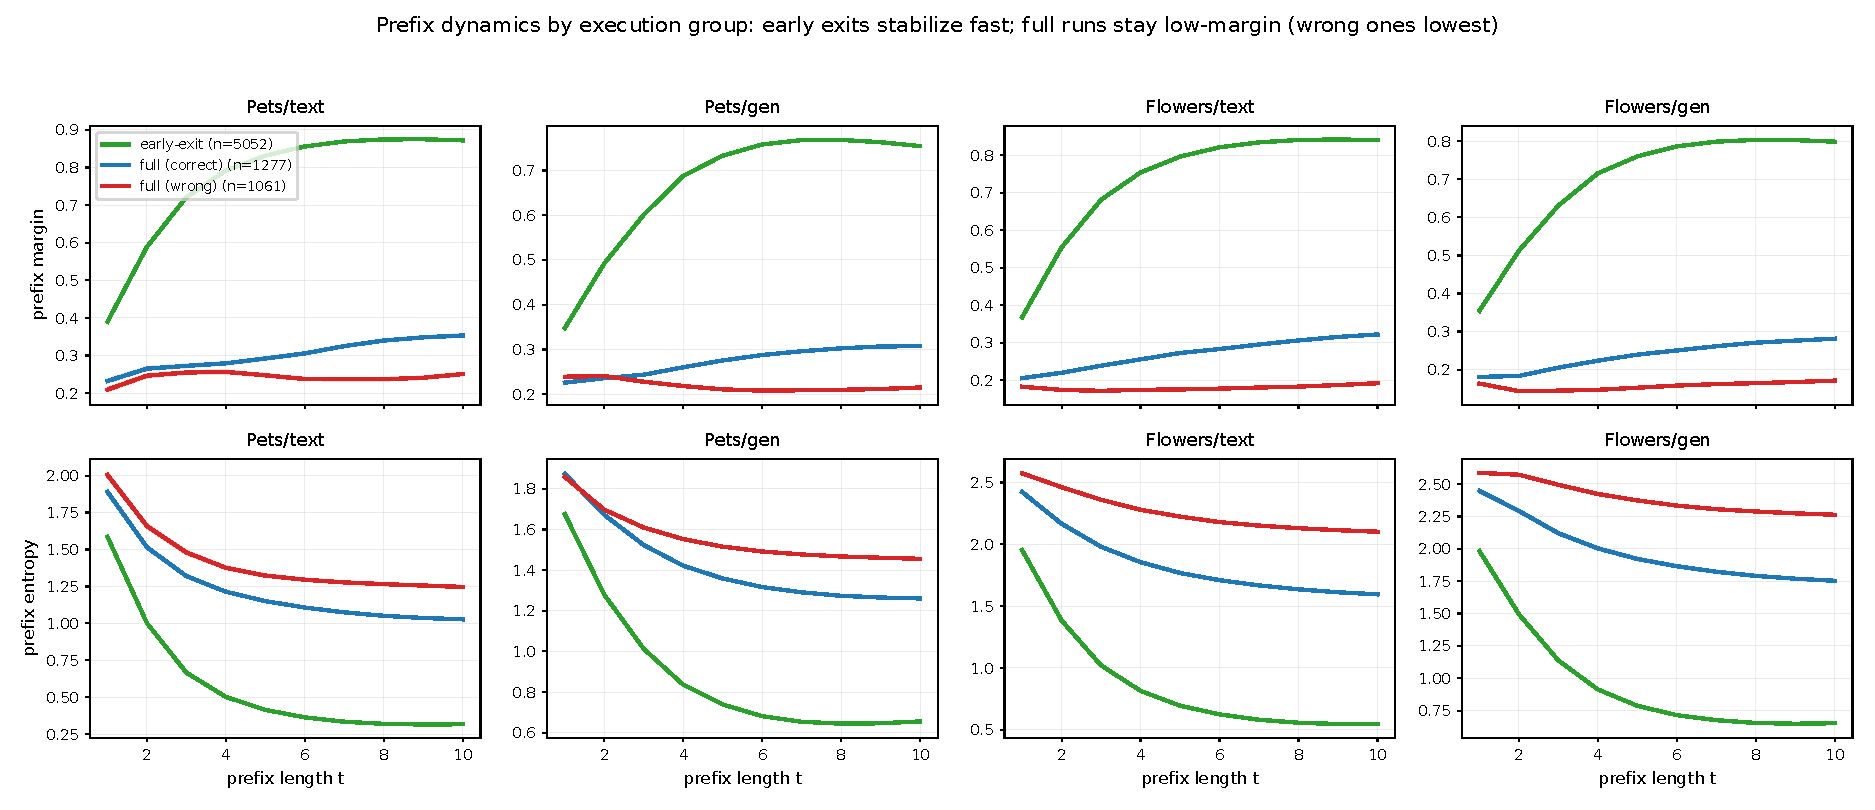
\includegraphics[width=0.98\linewidth]{figures/deep_diag/figT_trajectory.pdf}
\caption{Prefix margin (top) and entropy (bottom) trajectories by
execution group.}
\label{fig:traj}
\end{figure}

\paragraph{Symptom vs.\ signal: quadrant analysis and the drag statistic.}
Figure~\ref{fig:mech} reproduces the quadrant analysis of the main paper
(main Fig.~4). The
$s_1\times s_{10}$ correctness quadrants and the NQ-rescue rate. The
window between ``the fusion operator is beneficial'' and ``harmful''
domains is directly visible: rescue rates are 92--97\% on Pets/Flowers/CUB
but only 76--85\% on EuroSAT.
The label-free ``drag'' statistic --- over samples where $s_1$ and $s_{10}$
disagree, the fraction where the fused prediction follows $s_1$ --- shows
the same separation in the direction of displacement (18.4\% for
EuroSAT/gen vs.\ $\le 6.8\%$ elsewhere), but its regime separation
($+1.01$pp) is weaker than the entropy gap ($+2.20$pp), motivating the
entropy-based selector (Sec.~\ref{s:select}).

\paragraph{Attention statistics (negative result, reported for
completeness).}
A per-sample quantitative study of CLIP attention rollout (600 sampled
EuroSAT images $\times$ 10 scales) found the normalized attention entropy
to be nearly constant (all 12 layers $>0.91$; $0.998$ after rollout) and
uncorrelated with correctness or scale. CLIP attention is diffuse, so the
qualitative overlays in the main paper (main Fig.~3) are per-crop min--max
normalized for display; they are used to illustrate the
local-texture-to-global-structure transition, not as a quantitative
diagnostic. This negative result is why AdaScale uses prediction-space
statistics (entropy, margin, JS) rather than attention statistics.

\paragraph{Feature geometry.}
Figure~\ref{fig:geo} reports the mean cosine similarity to the ground-truth
prototype and the geometric margin
($\cos(f_s, p_{gt}) - \max_{c \ne gt}\cos(f_s, p_c)$) per scale. Alignment
increases with scale for all settings; synthetic prototypes plateau at a
lower geometric margin, consistent with their different calibration.

\begin{figure}[t]
\centering
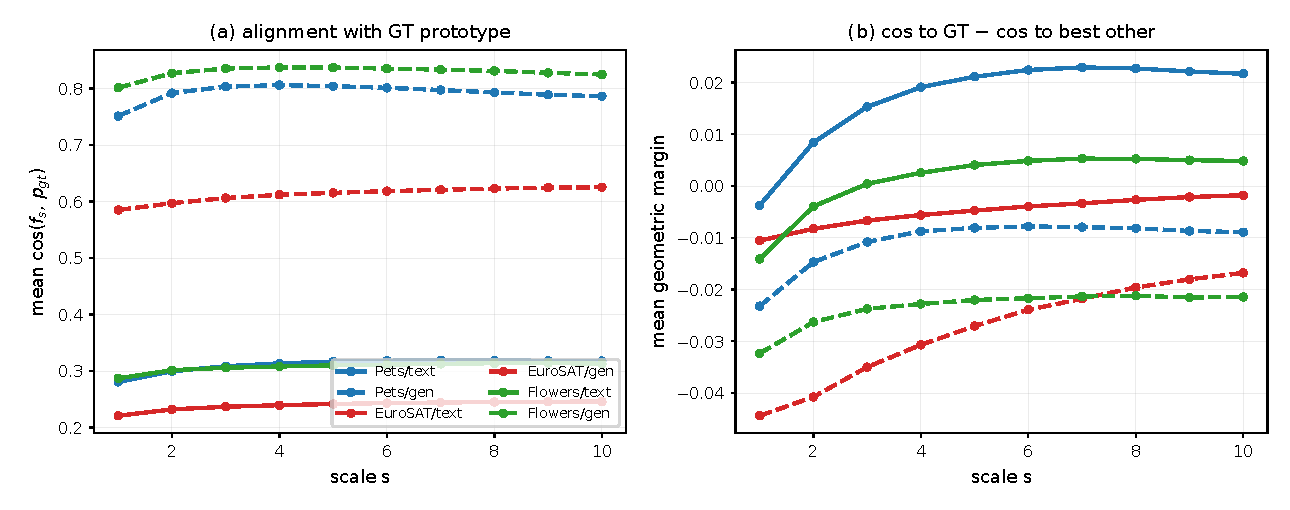
\includegraphics[width=0.85\linewidth]{figures/deep_diag/figG_geometry.pdf}
\caption{Feature geometry by scale.}
\label{fig:geo}
\end{figure}

\begin{figure}[t]
\centering
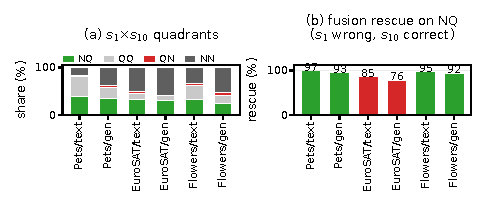
\includegraphics[width=0.8\linewidth]{figures/deep_diag/figM_compact.pdf}
\caption{Microscopic view of the domain-level fusion failure
(reproduced from the main paper, Fig.~4).}
\label{fig:mech}
\end{figure}

\section{Additional Results}
\label{s:extra}

\paragraph{ViT-B/16 full results.}
Table~\ref{tab:b16} reports all ViT-B/16 experiments. The selector is
correct on all four settings; AdaScale matches or exceeds Full-10 except
$0.04$ points on Pets/text (n.s.), with 15--90\% fewer scale evaluations.
Note the EuroSAT single-scale advantage reproduces exactly on the larger
backbone (42.74 vs.\ 40.47 fused).

\begin{table}[t]
\centering
\small
\caption{ViT-B/16 results. $\Delta H$: calibration entropy gap
(threshold $\theta{=}1\%$). v3: probability-level soft fusion.}
\label{tab:b16}
\begin{tabular}{llccccc}
\toprule
Setting & Mode & Full-10 & Single & v2 & v3 & \#Scales \\
\midrule
Pets/text & FUSED & 86.14 & 84.53 & 86.08 & {86.10} & 6.42 \\
Pets/gen  & FUSED & 64.17 & 61.96 & 64.15 & {64.49} & 8.50 \\
EuroSAT/text & SINGLE & 40.47 & 42.74 & 42.74 & — & 1.00 \\
Flowers/text & FUSED & 68.10 & 66.37 & 68.12 & {68.23} & 7.53 \\
\bottomrule
\end{tabular}
\end{table}

\paragraph{Runtime.}
Table~\ref{tab:runtime} (reproduced) reports wall-clock timings on a
single RTX 4080 Super, batch size 32, crops shared bit-exactly between
methods.

\begin{table}[t]
\centering
\caption{Wall-clock inference (batch 32, RTX 4080 Super). PET: $N{=}7390$; EuroSAT: $N{=}27000$; Single mode evaluates only the largest scale.}
\label{tab:runtime}
\small
\setlength{\tabcolsep}{4pt}
\begin{tabular}{lrrrr}
\hline
Method & Time (s) & Ips. & Acc (\%) & Avg. scales \\
\hline
Full-10 (PET) & 290 & 25.4 & 82.50 & 10.00 \\
Fixed-5 (PET) & 127 & 58.3 & 81.15 & 5.00 \\
Fixed-7 (PET) & 189 & 39.0 & 82.75 & 7.00 \\
AdaScale (PET) & 202 & 36.6 & 82.37 & 6.64 \\
Full-10 (EURO; 27k) & 397 & 68.0 & 42.35 & 10.00 \\
Single (EURO; 27k) & 45 & 595.8 & 45.34 & 1.00 \\
\hline
\end{tabular}
\end{table}


\paragraph{Soft-fusion ($v3$) sensitivity and gain decomposition.}
Across the eight fused-mode settings, probability-level soft fusion
improves accuracy by $+0.15$ on average (all non-negative; significant
on Flowers-102/gen $p{=}0.002$ and Pets/gen at ViT-B/16 $p{<}0.01$, n.s.\
elsewhere). The gain is fully attributable to hard samples: samples that
run to completion gain $+0.27$--$+0.56$, while early-exit samples change
by exactly $0.00$ (the decision layer is frozen, so runtime is unchanged).
Temperature sensitivity: $\tau_s \in \{0.01, 0.02, 0.05\}$ are all
non-negative, with $0.02$ most stable across settings.

\paragraph{Where fusion rescue degrades (mechanism).}
On EuroSAT, among samples where $s_1$ is wrong but $s_{10}$ is correct
(NQ, 33--38\% of the dataset), the fused predictor recovers only
84.6\%/76.2\% (text/gen, ViT-B/32) and 85.1\% (text, ViT-B/16), versus
92--97\% on all other datasets. This is the microscopic counterpart of
the domain-level failure and is reported in main Fig.~4.

\begin{thebibliography}{1}
\bibitem{shi2026lgclip} D.~Shi, D.~Fu, Y.~Liu, and J.~Wang, ``Can synthetic
images serve as effective and efficient class prototypes?,'' in \emph{ICASSP}, 2026.
\end{thebibliography}

\end{document}
